\chapter{Requirements}

\section{Roles}

Simple ODR platforms targeted towards e-commerce disputes typically involve just a buyer and a seller. Our ODR platform is intended to be applied to criminal law, thus having four main roles:

\begin{itemize}
\item \textbf{Law Firm} - a law firm, registered to the system by an authorised individual (such as managing director). A Law Firm can have many Agents.
\item \textbf{Agent} - a lawyer, working on behalf of the Law Firm. An Agent must be in one Law Firm.
\item \textbf{Mediation Centre} - a mediation centre, which is a company specialising in the mediation of disputes. A Mediation Centre can have many Mediators.
\item \textbf{Mediator} - a mediator, working on behalf of the Mediation Centre. A Mediator must be in one Mediation Centre.
\end{itemize}

\section{Use cases}

As with all requirements specifications, a good place to begin was to create various use case diagrams representing the roles in the system and the actions they ought to be able to perform. By doing so, it would also be possible to derive common classes and actions by examining similar or duplicating use case scenarios. These use cases were derived from early meetings with the client and other stakeholders, where they discussed in detail how the process of online dispute resolution should be applied.

\subsection{Registration}

\begin{figure}[h!]
  \centering
    \ifimages
    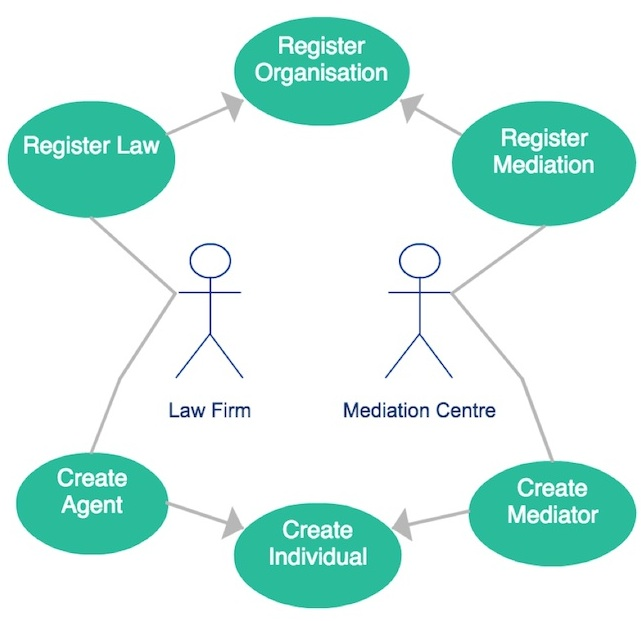
\includegraphics[width=0.7\textwidth]{use_case--registration}
    \fi
  \caption{Use case diagram showing registration feature}
  \label{uml:useCase:registration}
\end{figure}

Authorised individuals should be allowed to register accounts representing their company (be it a law firm or mediation centre), and within that organisation account they should be able to register individual accounts. These individual accounts should be agents or mediators depending on the organisation type.

Figure~\ref{uml:useCase:registration} shows this in terms of the law firms and mediation centres. A generalised action has been added in both the organisation and individual registration, showing where it might be possible to use a common class or database table to accomplish both goals.

\subsection{Disputes}

\begin{figure}[h!]
  \centering
    \ifimages
    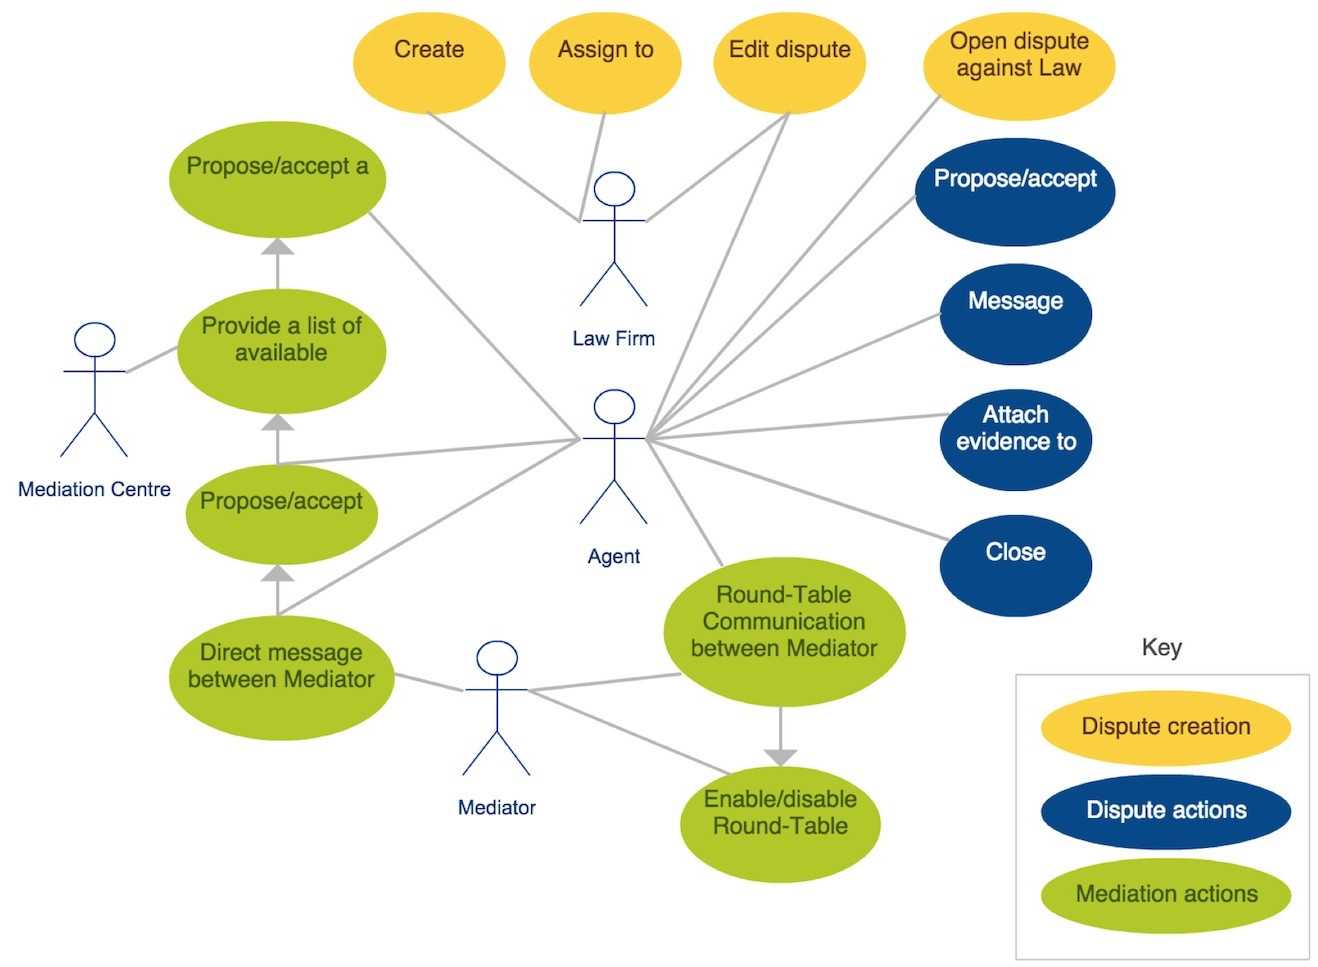
\includegraphics[width=\textwidth]{use_case--disputes}
    \fi
  \caption{Use case diagram showing actions available in a dispute}
  \label{uml:useCase:disputes}
\end{figure}

Figure~\ref{uml:useCase:disputes} shows the roles and actions involved in the creation, mediation and closing of a dispute. Arrows denote where one action has a dependency on another.

Only law firms can create new disputes. There is then some back-and-forth assignment between law firms and agents until both sides of a dispute are represented by opposing agents. This is identified as being the `dispute creation' stage.

Inside a dispute, agents should be able to negotiate the dispute lifespan, exchange messages and evidence, and should have the freedom to close a dispute. In a best-case scenario, this is all that is required to successfully resolve a dispute. This is known as the `dispute' stage.

Should it be required, an agent can propose mediation, and there is a defined process of administration between the agents and mediation centre required to get the dispute `in mediation'. Once in this state, the agents can communicate only through the mediator, unless the mediator feels the dispute is close to resolution and decides to enable round-table communication.

\subsection{Miscellaneous}

\begin{figure}[h!]
  \centering
    \ifimages
    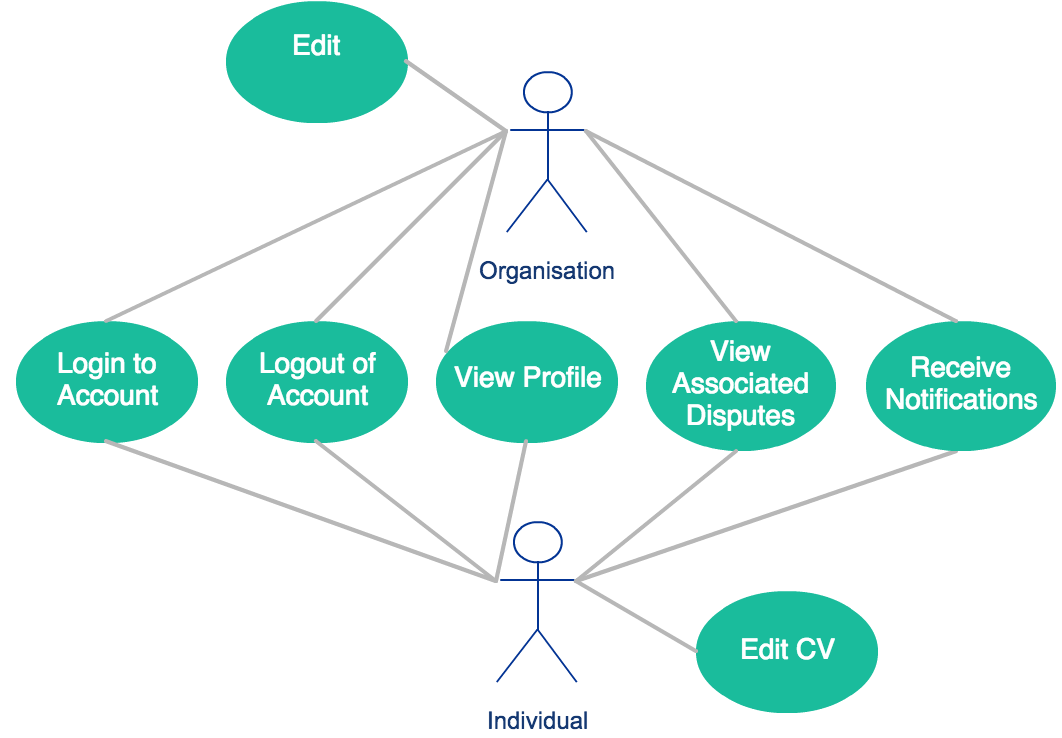
\includegraphics[width=0.9\textwidth]{use_case--miscellaneous}
    \fi
  \caption{Use case diagram demonstrating other miscellaneous requirements}
  \label{uml:useCase:miscellaneous}
\end{figure}

Other, lesser elements of functionality are shown by the miscellaneous UML diagram in figure~\ref{uml:useCase:miscellaneous}. For example, agents should be able to peruse a mediator's CV before making a decision as to which mediator to opt for. This suggests the need for a ``view profile" facility with custom fields for the CV, which could be as simple as a HTML textarea or as complicated as an integrated PDF uploader and viewer.

Given the tight deadline of the project and the scale of the system, coupled with the high priority of demonstrating some maritime collision logic, it was decided that these miscellaneous features should be kept as simple as possible.

\section{Dispute process}

Although the use case diagrams describe the features required by the system, they do not make it very clear when those features should or should not be available. An early meeting with the client emphasised that a dispute should follow a very specific workflow.

\begin{figure}[h!]
  \centering
    \ifimages
    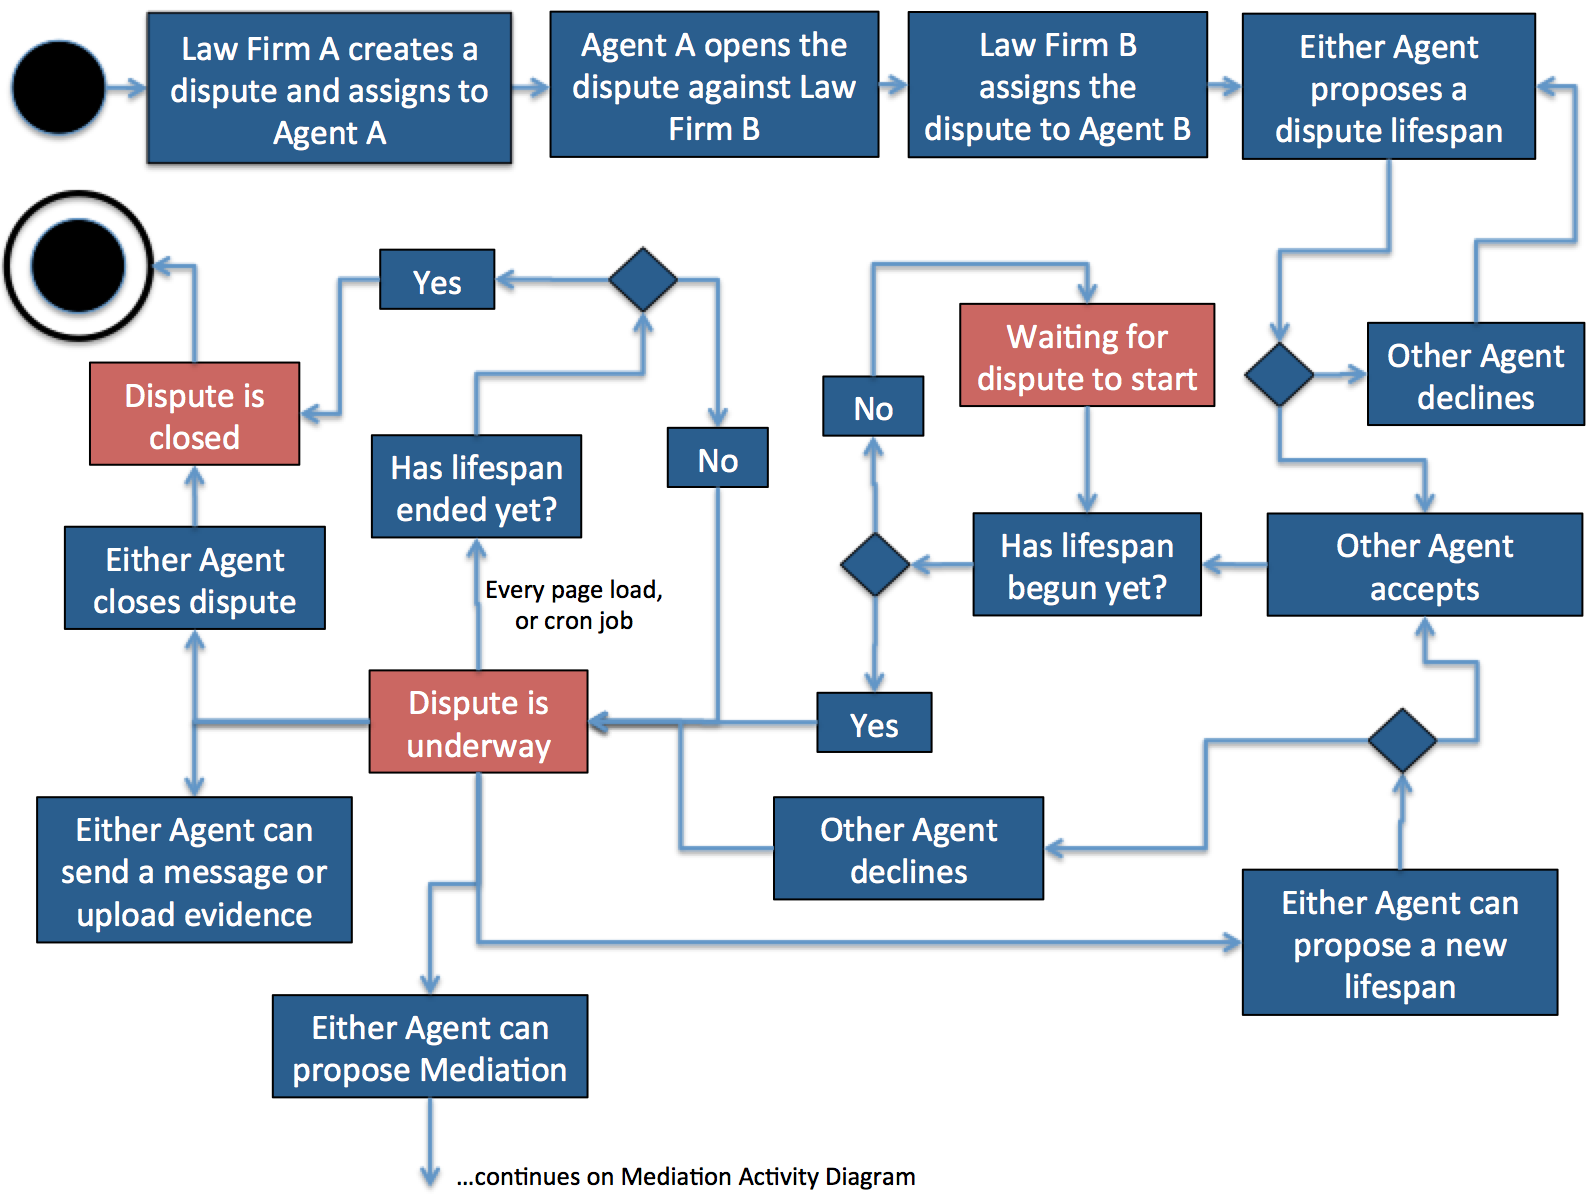
\includegraphics[width=\textwidth]{dispute_process}
    \fi
  \caption{Activity diagram showing the workflow required in creating a dispute}
  \label{uml:activity:dispute}
\end{figure}

The activity diagram in figure~\ref{uml:activity:dispute} shows the creation of a dispute and the features that become available to the agents when the dispute has been initialised. The red boxes indicate the current `state' of the dispute. The activity diagram continues into figure~\ref{uml:activity:mediation}, which shows what is involved in putting a dispute into mediation. Again, red boxes indicate dispute state.

\begin{figure}[h!]
  \centering
    \ifimages
    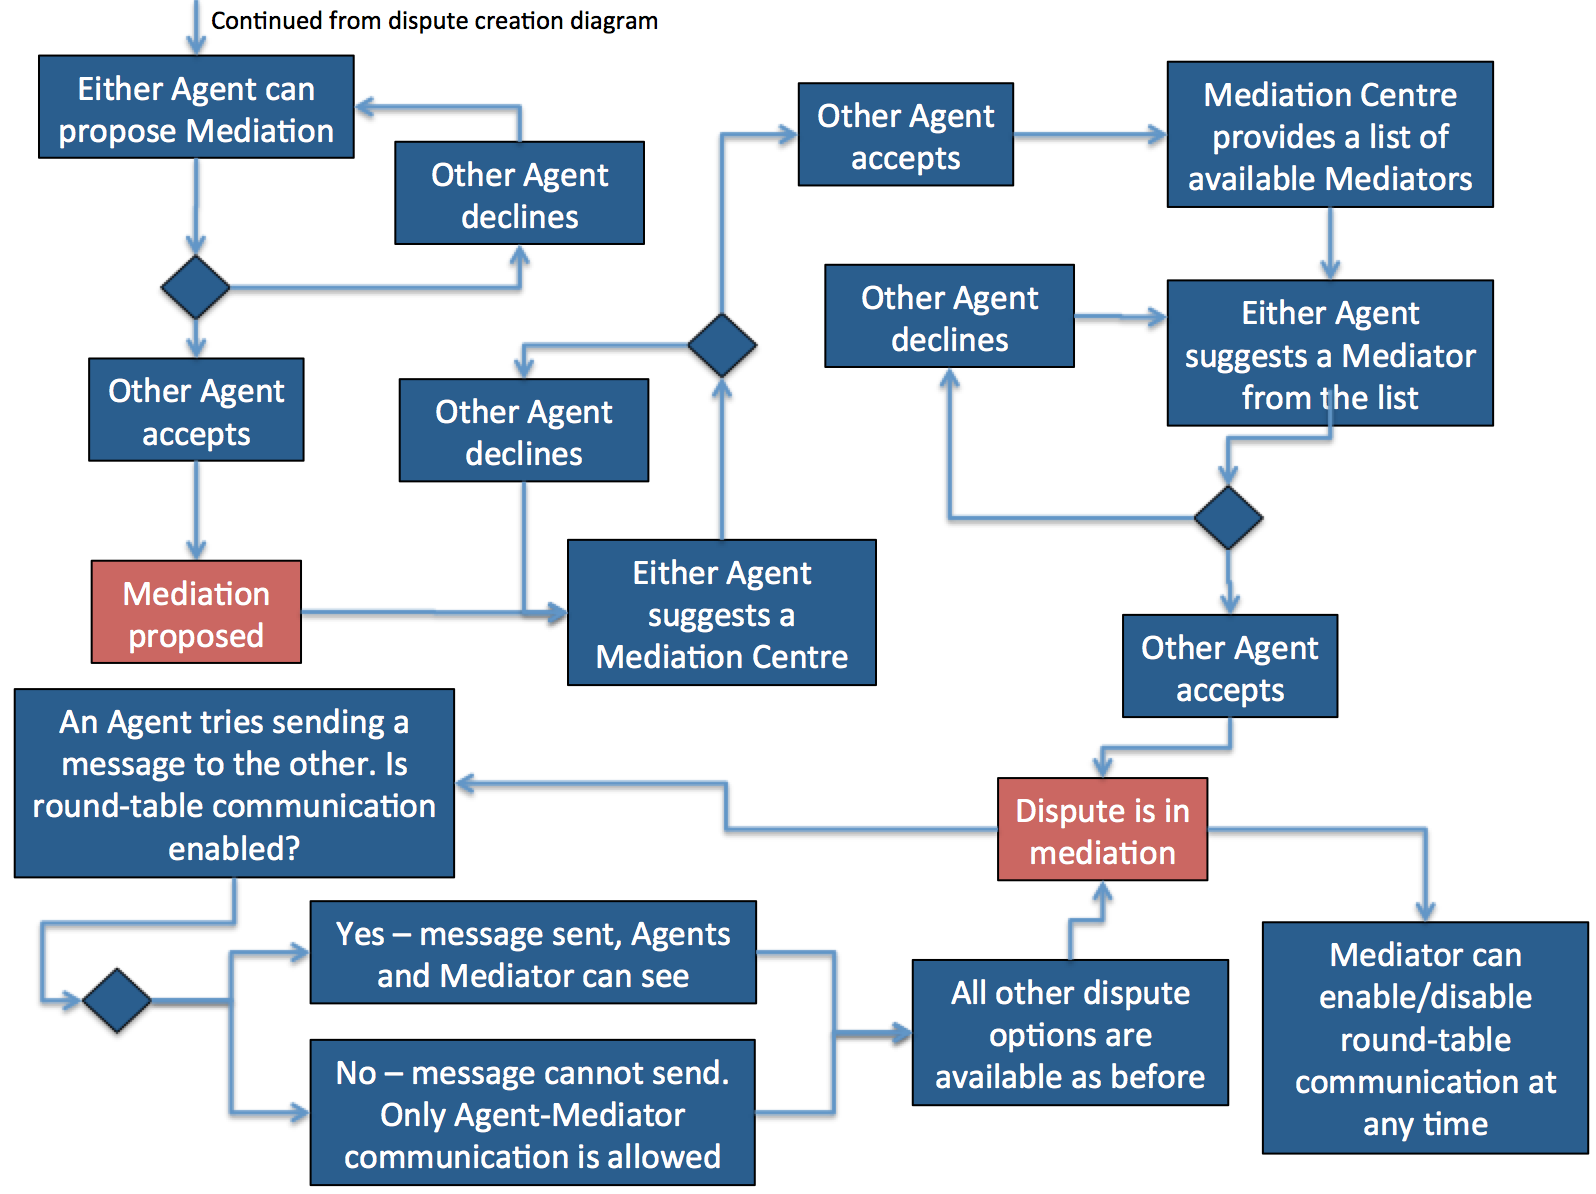
\includegraphics[width=\textwidth]{dispute_process--mediation}
    \fi
  \caption{Activity diagram showing the workflow involved in getting a dispute into mediation}
  \label{uml:activity:mediation}
\end{figure}

\section{Features}

Following on from the use case diagrams, it was critical to explicitly define the project requirements in a textual way. In a traditional Waterfall model, a requirements specification is a key deliverable created at the beginning of the process, whereas in an agile model, features are represented as user stories which are then estimated, prioritised and tackled incrementally.

Before immortalising the requirements in a textual form, a project development approach had to be decided upon.

\subsection{Project Development Methodology}

The industry is moving towards an agile approach [REF] which stresses the importance of being able to embrace change. As Kent Beck once said, agile is about ``deferring design decisions until the last possible moment so that they can be made in light of experience" gained through spike work, talking to the on-site customer, and so on.

The idea of agile is that the cost-of-change curve is made shallower. Customers are happy because it's never too late to tweak a feature, and developers are happy because they're not expending lots of effort into writing up requirements specifications, designing UML diagrams, and the like.

Numerous high-profile examples exist of multi-million pound software systems going exponentially over budget or failing to deliver at all as a result of following the Waterfall model, which some consider to be antiquated and not suited to the world of software engineering. In comparison, there is this image of agile developers being able to nimbly build incredible systems without being held up by dull and costly processes such as documentation.

We should be able to adapt our choice of methodology to the project at hand, not the project at hand to our choice of methodology. Looking at this project impartially, I had a few reasons to consider a plan-driven approach:

\begin{itemize}

    \item This project requires building an Online Dispute Resolution system. Systems like this have already been established, meaning that there is already a list of fairly straightforward features that can be formalised in advance to be taken into account in the design.
    
    \item In ODR, there is a heavy emphasis on law and following processes correctly. For example, the ODR platform cannot be allowed to give either party an unfair advantage through being able to exploit lifespan negotiation. It is absolutely critical that the platform does not violate any of the rules of ODR - and therefore it is essential to document these rules in the requirements specification, for traceability and accountability.
    
    \item This project's customer is very busy and has only been able to meet a couple of times over the course of the project. This is not nearly often enough to constitute as an `on-site customer' - one of the pre-requisites of an agile project - again suggesting that plan-driven is the best approach.
    
    \item Finally, the process of gathering requirements, creating a design, and implementing and testing a substantial software system is still somewhat new to the sole developer on this project. Having a design and a plan is a comforting safety net.

\end{itemize}

Of course, the above points don't disqualify agile practices from the project. Agile principles of TDD, continuous integration (CI), regular releases and merciless refactoring are all very worthwhile activities and are not necessarily mutually exclusive from the Waterfall model. However, they do not lend themselves particularly well to the traditional workflow of implementation and then testing.

Thus, it was decided that the approach should be a hybrid one of Waterfall and Agile. The project should begin with a strong set of requirements and there should be some up front design for parts of the project that are unlikely to change, such as the database schema. At the implementation stage, the project should switch to a business-driven, test-driven approach that utilises the best of the agile processes.

\subsection{Textualising Requirements}

My approach to textualising requirements is a compromise between plan-driven and agile approaches. In this project, I specified requirements in the form of Cucumber features.

In agile approaches, user stories should be the simplest thing to make everyone in the room agree that there is a placeholder for something that needs to be done. In plan-driven approaches, requirements are specified by way of a fully comprehensive report in the form of a detailed requirements specification. Cucumber features are the middle ground: more detailed than user stories, but executable in a BDD approach that lends itself perfectly to the agile practices of TDD and CI.

BDD, or business-driven development, allows you to write features in a human-readable way so that a business analyst is able to understand the requirements but does not need to know the technical implementation. The features follow a convention known as the Gherkin syntax [REF] so that each feature step can be matched to a corresponding step definition represented in code. This makes the features executable and allows automated end-to-end testing.

Appendix~\ref{appendix:requirements} contains the full set of Cucumber features, which form the basis of the requirements specification. They're more useful than a traditional specification as they can be `run' to ensure that the requirements have been met. The nature of these being a part of the codebase means that they can evolve over time, which is simultaneously an advantage and a disadvantage. For this reason, appendix~\ref{appendix:requirements} contains the set of original signed-off features plus the final set of features as they now stand at the end of the project.

\subsection{Development Methodology versus Project Management}

Each of the development methodologies discussed has an associated project management approach. Waterfall projects tend to use Gantt charts to plan progress, whereas agile approaches tend to use sprints to plan individual iterations. As this project will be using a hybrid development methodology, the question was raised as to whether or not it should be using a hybrid project management approach.

Given that the first half of the project would be plan-driven and that significant efforts were made in the early stages of the project to clarify exact requirements, it made sense to adopt the plan-driven approach of creating a Gantt chart which plans out the implementation of the features.

\begin{figure}[h!]
  \centering
    \ifimages
    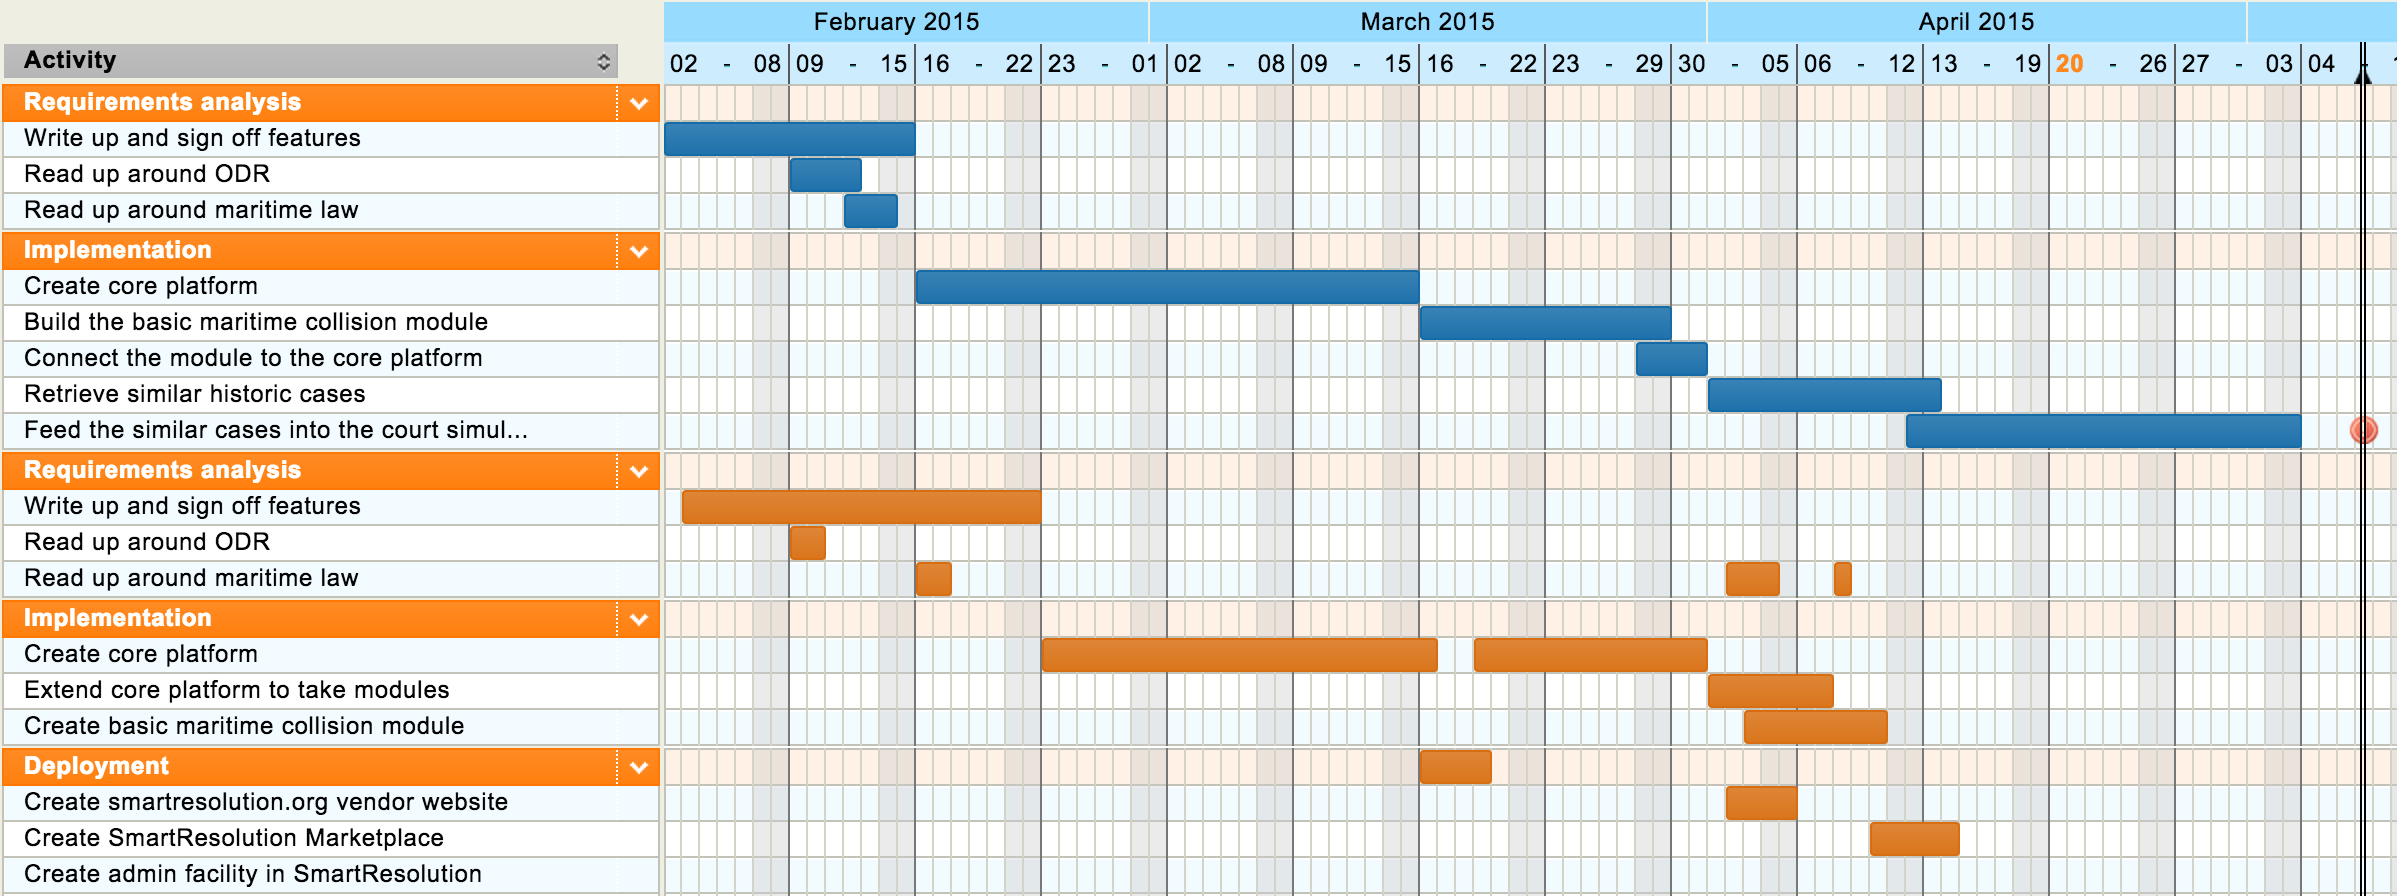
\includegraphics[width=1.4\textwidth,angle =90]{gantt}
    \fi
  \caption{Gantt chart showing the original plan, compared with the plan actually followed}
  \label{uml:gantt}
\end{figure}

The Gantt chart in figure~\ref{uml:gantt} shows two timelines. The time periods in blue represent the original Gantt chart I intended to follow for this project. The time periods in orange represent what actually happened over the course of the project. The reasons for the disparities between the two are discussed in the evaluation section.

\section{SmartResolution}

The report thus far has discussed the project in the form of two main components: the core ODR platform, and the maritime collision module. Realistically, a third component was required: a vendor website. At the very least, this website would host the core software and provide instructions on how to install it onto a server. Additionally, it should host the maritime collision module and provide instructions describing how to install it onto the core platform.

If developers were to be excited enough about the ODR possibilities to develop modules of functionality like the maritime collision module, then this project would require a brand. I felt that the term `SmartResolution' embodied what the ODR platform was all about: online dispute resolutions done in a smart way, through interpreting disputes using artificial intelligence and automatically suggesting resolutions. This is the term I'll use to refer to the core platform from this point onwards.

Far from being just an information resource, I hoped that the SmartResolution website would also provide a facility to download and install SmartResolution modules directly through the SmartResolution installation itself, a little like downloading an app to an Android device directly through the Google Play store. Originally just an idea, this later fed into the revised requirements and was implemented towards the end of the project.